\documentclass[border=8pt]{standalone}
\usepackage{tikz}
\usetikzlibrary{arrows.meta, positioning, shapes.geometric}
\begin{document}
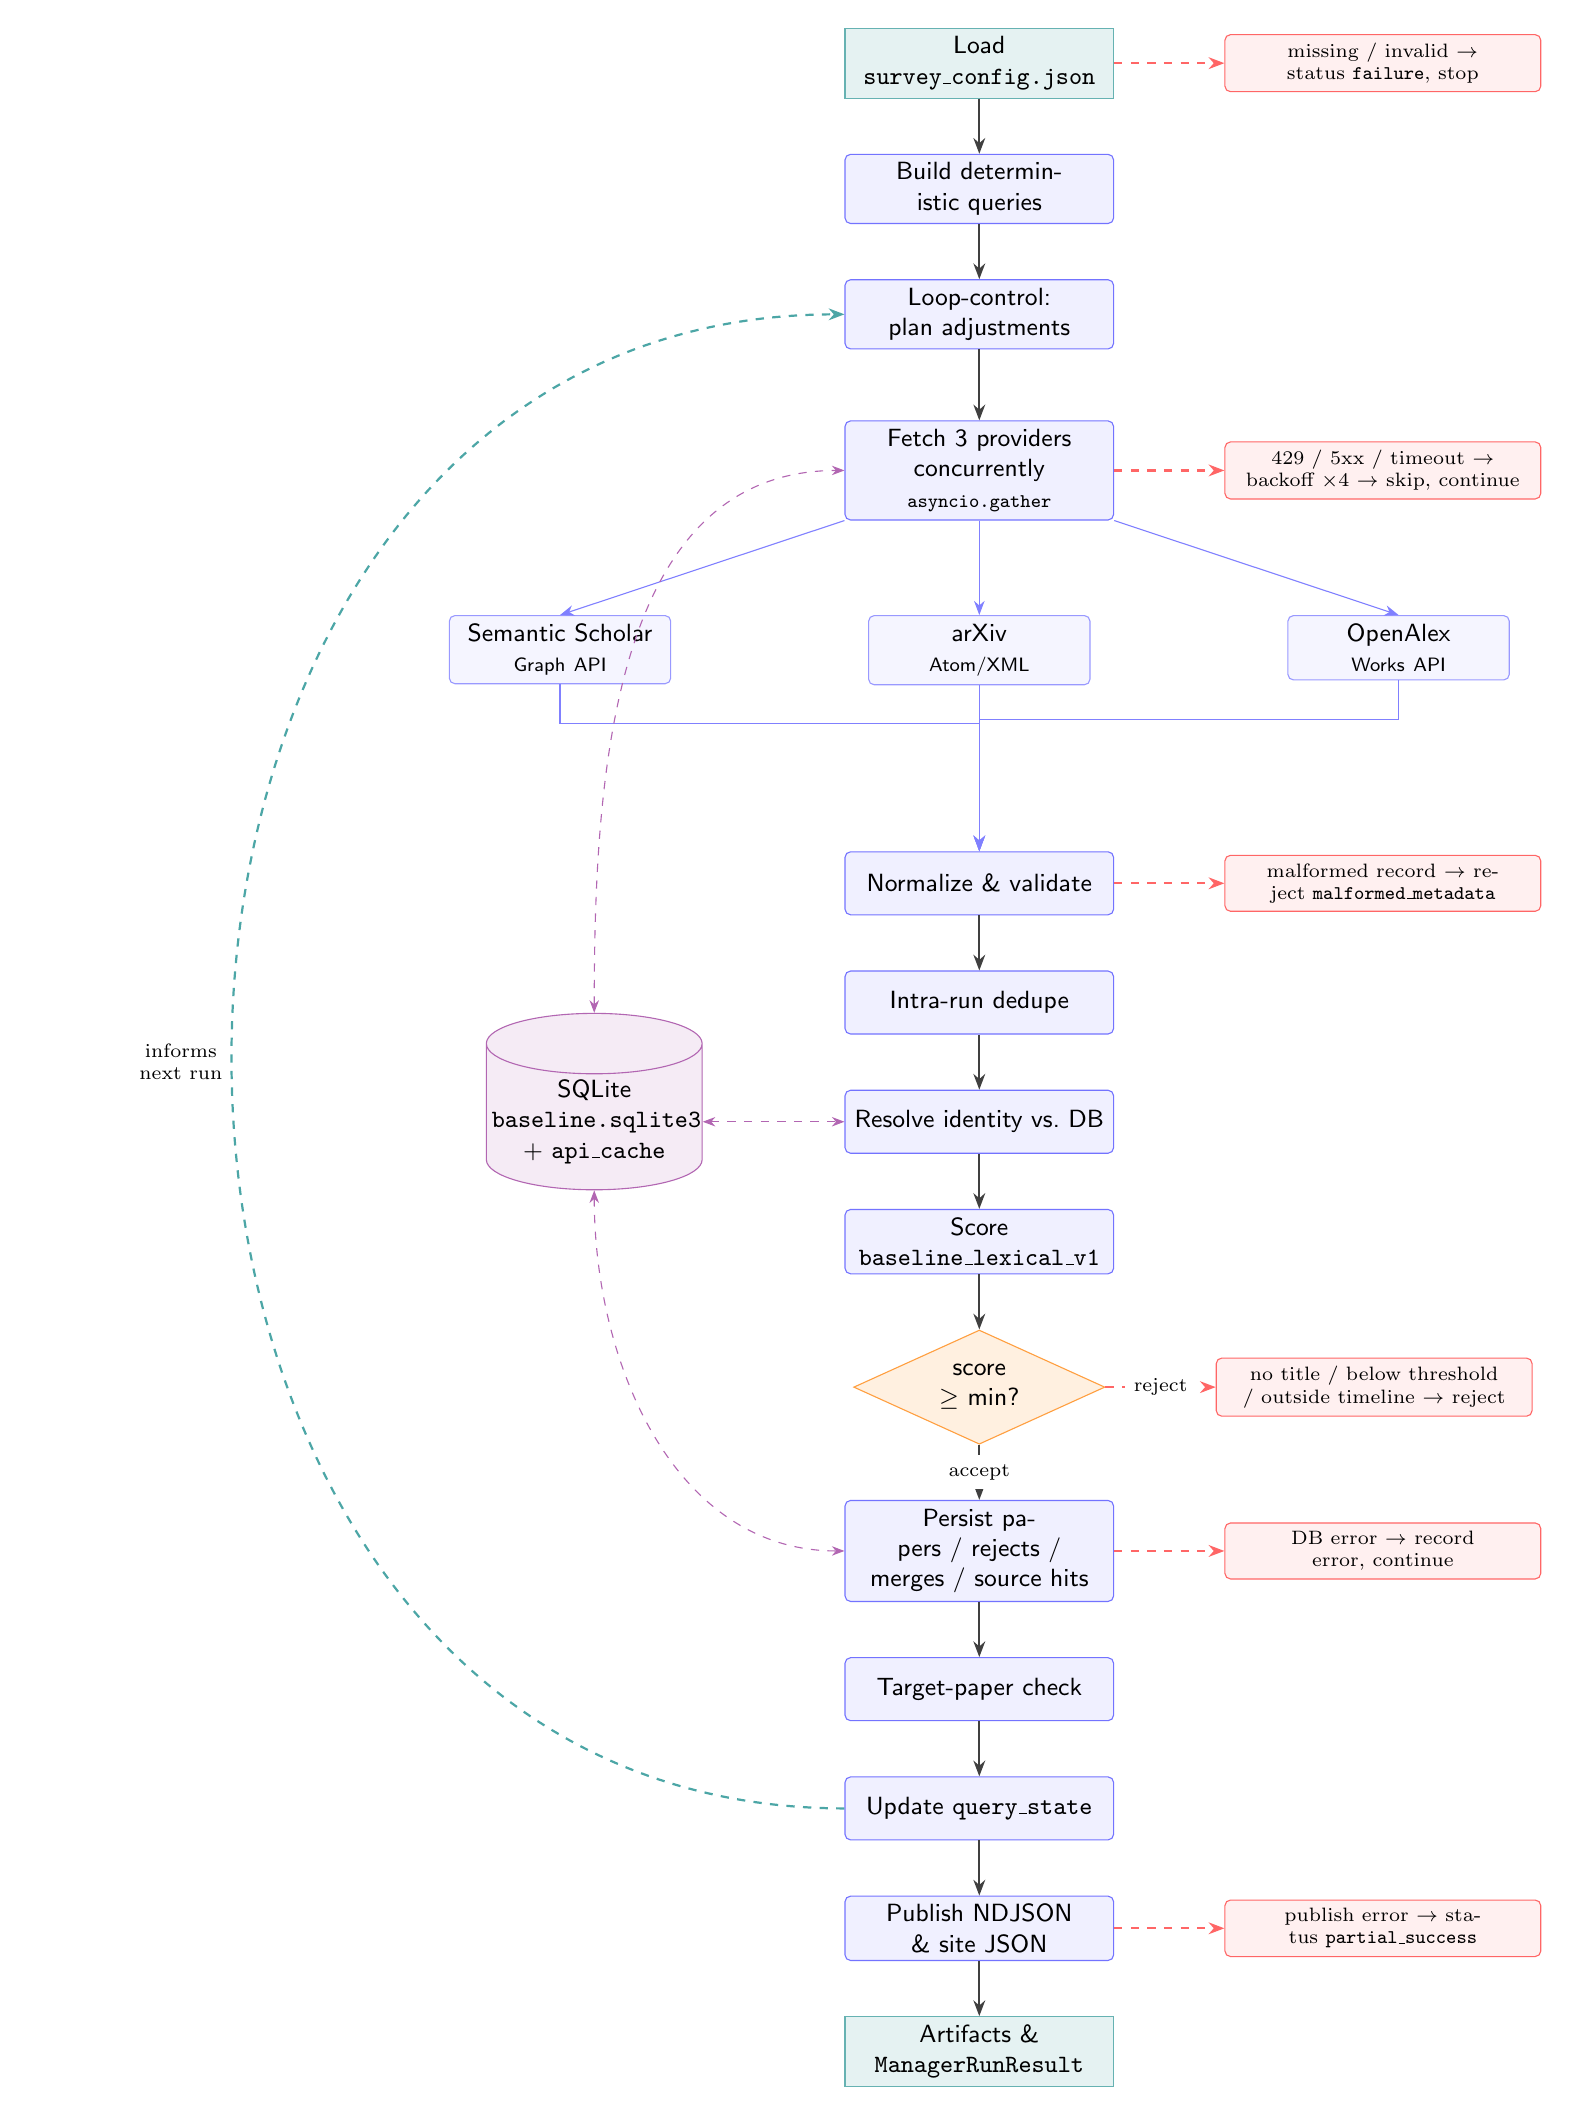
\begin{tikzpicture}[
  font=\small\sffamily,
  node distance=7mm and 18mm,
  proc/.style ={rectangle, rounded corners=2pt, draw=blue!55, fill=blue!6,
                text width=32mm, align=center, minimum height=8mm, inner sep=3pt},
  prov/.style ={rectangle, rounded corners=2pt, draw=blue!40, fill=blue!4,
                text width=26mm, align=center, minimum height=8mm, inner sep=3pt},
  io/.style   ={rectangle, draw=teal!60, fill=teal!10,
                text width=32mm, align=center, minimum height=8mm, inner sep=3pt},
  dec/.style  ={diamond, aspect=2.2, draw=orange!75, fill=orange!12,
                text width=17mm, align=center, inner sep=1pt},
  store/.style={cylinder, shape border rotate=90, aspect=0.28, draw=violet!60,
                fill=violet!8, text width=26mm, align=center, minimum height=12mm,
                inner sep=2pt},
  fail/.style ={rectangle, rounded corners=2pt, draw=red!60, fill=red!6,
                text width=38mm, align=center, font=\scriptsize, inner sep=3pt},
  flow/.style ={-{Stealth[length=2mm]}, thick, draw=black!75},
  pflow/.style={-{Stealth[length=1.8mm]}, draw=blue!50},
  soft/.style ={-{Stealth[length=2mm]}, thick, dashed, draw=red!60},
  link/.style ={{Stealth[length=1.6mm]}-{Stealth[length=1.6mm]}, dashed, draw=violet!60},
  back/.style ={-{Stealth[length=2mm]}, thick, dashed, draw=teal!70},
  gather/.style={-{Stealth[length=2mm]}, draw=blue!50},
]

% ---- happy-path spine ----
\node[io]                     (cfg)  {Load \texttt{survey\_config.json}};
\node[proc, below=of cfg]     (q)    {Build deterministic queries};
\node[proc, below=of q]       (plan) {Loop-control: plan adjustments};

% concurrent provider fetch
\node[proc, below=9mm of plan] (gather) {Fetch 3 providers concurrently\\{\scriptsize\texttt{asyncio.gather}}};

\node[prov, below left=12mm and 22mm of gather]  (s2)  {Semantic Scholar\\{\scriptsize Graph API}};
\node[prov, below=12mm of gather]                (ax)  {arXiv\\{\scriptsize Atom/XML}};
\node[prov, below right=12mm and 22mm of gather] (oa)  {OpenAlex\\{\scriptsize Works API}};

\node[proc, below=42mm of gather] (nv)  {Normalize \& validate};
\node[proc, below=of nv]          (dd)  {Intra-run dedupe};
\node[proc, below=of dd]          (rs)  {Resolve identity vs.\ DB};
\node[proc, below=of rs]          (sc)  {Score \texttt{baseline\_lexical\_v1}};
\node[dec,  below=of sc]          (ft)  {score $\ge$ min?};
\node[proc, below=of ft]          (ps)  {Persist papers / rejects /\\merges / source hits};
\node[proc, below=of ps]          (tc)  {Target-paper check};
\node[proc, below=of tc]          (qs)  {Update \texttt{query\_state}};
\node[proc, below=of qs]          (pb)  {Publish NDJSON \& site JSON};
\node[io,   below=of pb]          (rt)  {Artifacts \& \texttt{ManagerRunResult}};

% ---- local data store ----
\node[store, left=18mm of rs] (db) {SQLite\\\texttt{baseline.sqlite3}\\+ \texttt{api\_cache}};

% ---- fail-soft handlers (right column) ----
\node[fail, right=14mm of cfg]    (e1) {missing / invalid $\rightarrow$ status \texttt{failure}, stop};
\node[fail, right=14mm of gather] (e2) {429 / 5xx / timeout $\rightarrow$ backoff $\times$4 $\rightarrow$ skip, continue};
\node[fail, right=14mm of nv]     (e3) {malformed record $\rightarrow$ reject \texttt{malformed\_metadata}};
\node[fail, right=14mm of ft]     (e4) {no title / below threshold / outside timeline $\rightarrow$ reject};
\node[fail, right=14mm of ps]     (e5) {DB error $\rightarrow$ record error, continue};
\node[fail, right=14mm of pb]     (e6) {publish error $\rightarrow$ status \texttt{partial\_success}};

% ---- main flow ----
\draw[flow] (cfg)--(q);
\draw[flow] (q)--(plan);
\draw[flow] (plan)--(gather);

% fan out to providers
\draw[pflow] (gather.south west) -- (s2.north);
\draw[pflow] (gather.south)      -- (ax.north);
\draw[pflow] (gather.south east) -- (oa.north);

% fan in from providers
\draw[gather] (s2.south) -- ++(0,-5mm) -| (nv.north);
\draw[gather] (ax.south) -- (nv.north);
\draw[gather] (oa.south) -- ++(0,-5mm) -| (nv.north);

\draw[flow] (nv)--(dd);
\draw[flow] (dd)--(rs);
\draw[flow] (rs)--(sc);
\draw[flow] (sc)--(ft);
\draw[flow] (ft)--(ps) node[midway, fill=white, font=\scriptsize] {accept};
\draw[flow] (ps)--(tc);
\draw[flow] (tc)--(qs);
\draw[flow] (qs)--(pb);
\draw[flow] (pb)--(rt);

% ---- soft / error edges ----
\draw[soft] (cfg)--(e1);
\draw[soft] (gather)--(e2);
\draw[soft] (nv)--(e3);
\draw[soft] (ft)--(e4) node[midway, fill=white, font=\scriptsize] {reject};
\draw[soft] (ps)--(e5);
\draw[soft] (pb)--(e6);

% ---- data-store links ----
\draw[link] (db.north) to[out=90,in=180]  (gather.west);
\draw[link] (db.east)  --                  (rs.west);
\draw[link] (db.south) to[out=-90,in=180]  (ps.west);

% ---- feedback loop ----
\draw[back] (qs.west) to[out=180,in=180,looseness=1.4]
      node[left, align=center, font=\scriptsize] {informs\\next run} (plan.west);

\end{tikzpicture}
\end{document}
